\documentclass[11pt]{article}
\usepackage[a4paper,margin=23mm]{geometry}
\usepackage{amsmath,amssymb,amsthm,mathtools}
\usepackage{graphicx}
\usepackage{microtype}
\usepackage{xcolor}
\usepackage[colorlinks=true,linkcolor=blue!55!black,citecolor=blue!55!black,urlcolor=blue!55!black]{hyperref}

\newtheorem{theorem}{Theorem}
\newtheorem{lemma}[theorem]{Lemma}
\newtheorem{corollary}[theorem]{Corollary}
\newcommand{\W}{\mathcal W}
\newcommand{\C}{\mathbb C}
\newcommand{\F}{\mathbb F}
\newcommand{\tr}{\operatorname{tr}}
\newcommand{\conv}{\operatorname{conv}}

\title{The Exact SD-Tuple Boundary Is Reciprocal $\ell^1$\\
\large Mutually unbiased bases determine the uniform SD-constant}
\author{Candidate full result for the SD-tuple question in arXiv:1803.09212}
\date{13 August 2026}

\begin{document}
\maketitle

\begin{center}
\fbox{\parbox{0.92\linewidth}{\textbf{Status: candidate full proof, likely valid.}
The packet resolves the precise SD-tuple classification question and computes
the uniform SD-constant.  It does not solve the source's broader product
containment Problem~2.3.  Novelty remains subject to expert literature review.}}
\end{center}

\section{Source question and exact scope}

Passer defines the standard simplex
$\Delta_n=\conv\{0,e_1,\ldots,e_n\}$ and the standard diamond
$\Diamond_n=\conv\{\pm e_1,\ldots,\pm e_n\}$, and then introduces
SD-tuples on source PDF p.~7 \cite{Passer}:

\begin{center}
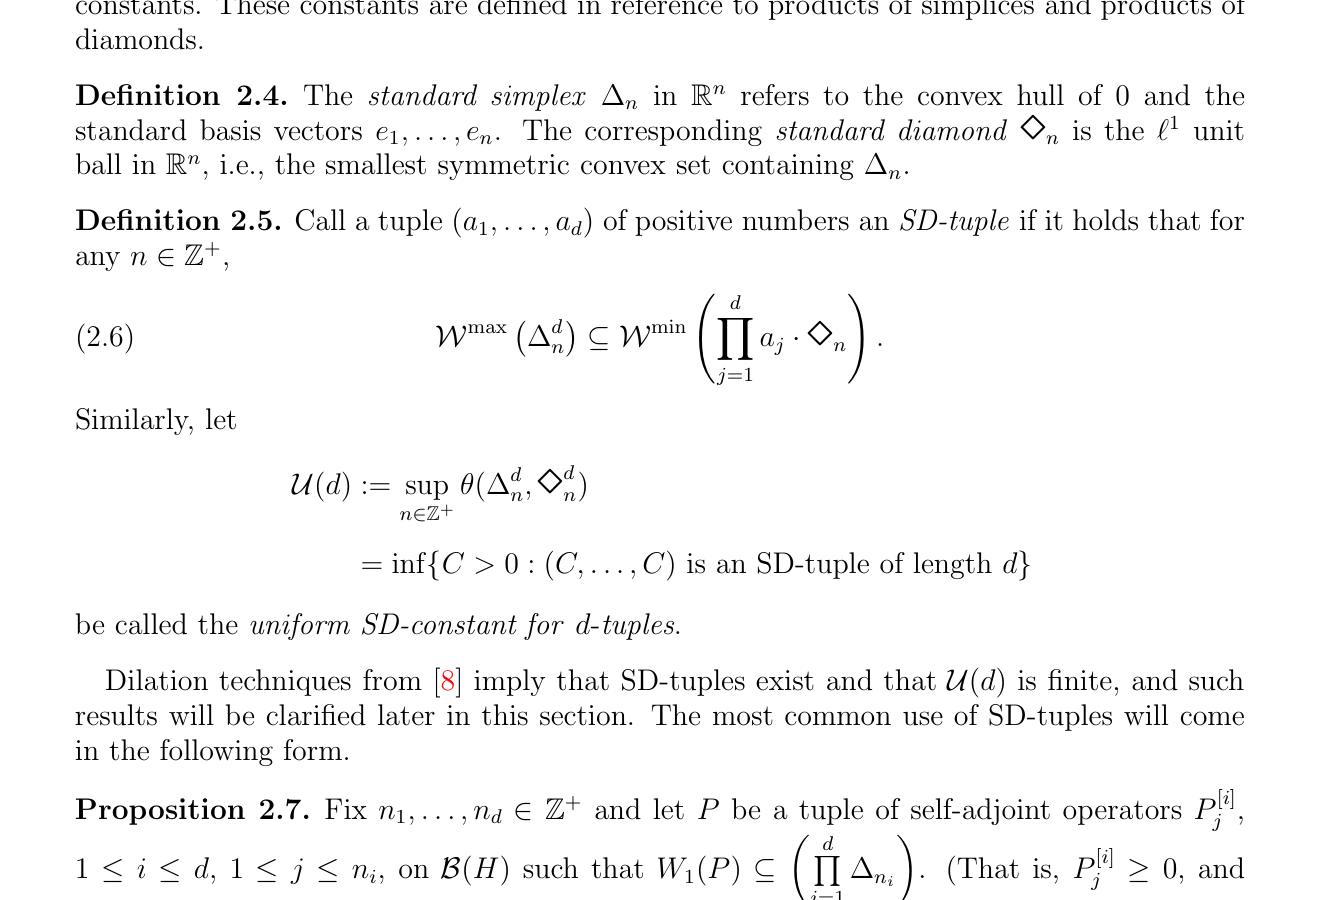
\includegraphics[width=0.96\linewidth]{figures/sd_definition_crop.png}
\end{center}

\noindent\textbf{Exact transcription of Definition 2.5.}
``Call a tuple $(a_1,\ldots,a_d)$ of positive numbers an SD-tuple if it
holds that for any $n\in\mathbb Z^+$,
\[
 \W^{\max}(\Delta_n^d)\subseteq
 \W^{\min}\!\left(\prod_{j=1}^d a_j\cdot\Diamond_n\right).
\]''
The uniform SD-constant is
\[
 \mathcal U(d)=\inf\{C>0:(C,\ldots,C)\text{ is an SD-tuple of length }d\}.
\]

The source proves a reciprocal $\ell^1$ sufficient condition and a reciprocal
$\ell^2$ necessary condition, leaving the gap shown on source PDF p.~11:

\begin{center}
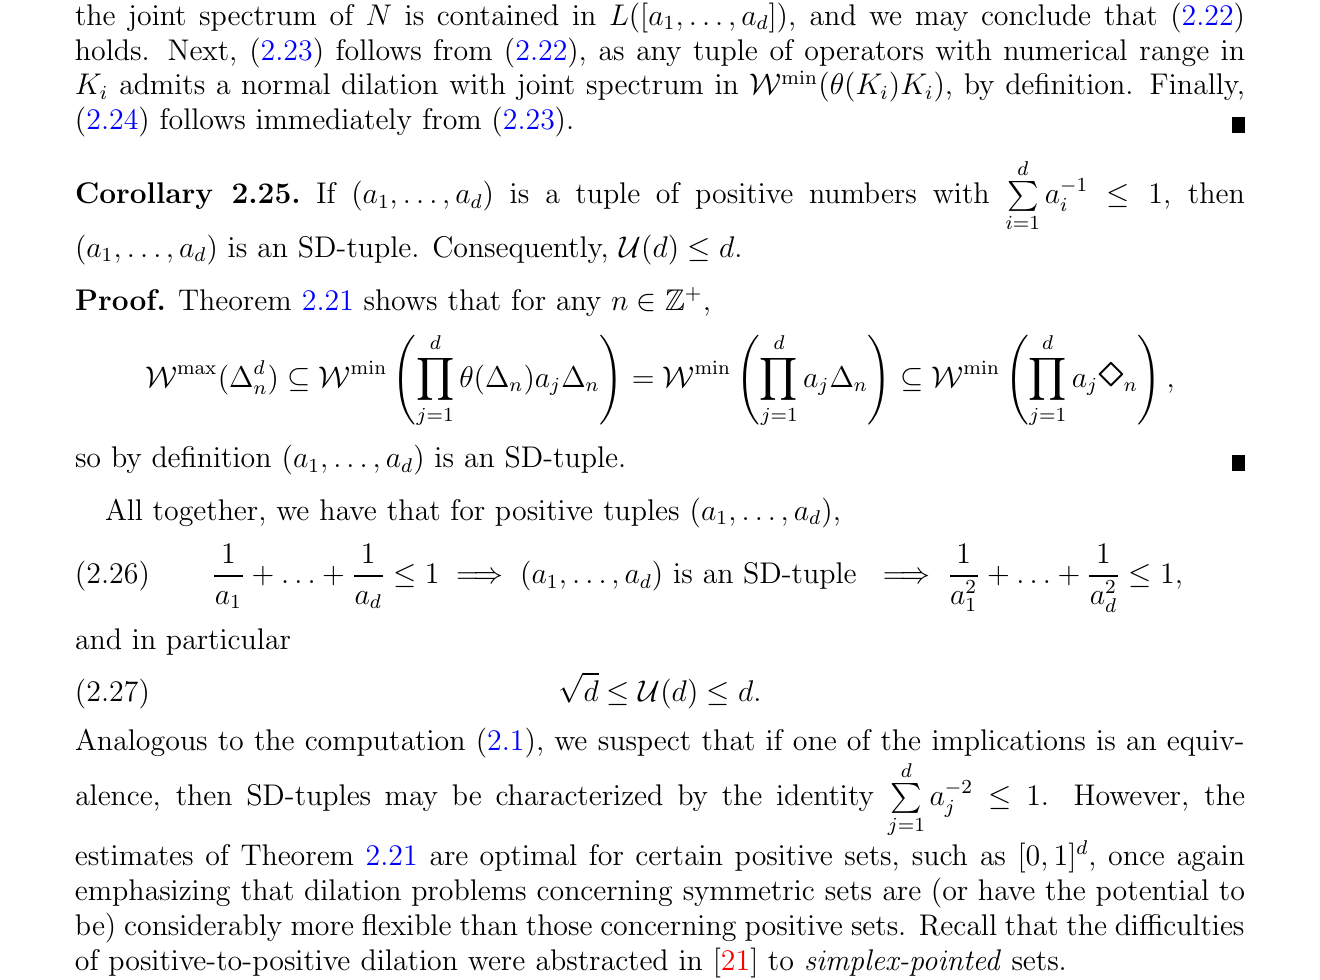
\includegraphics[width=0.96\linewidth]{figures/sd_question_crop.png}
\end{center}

\noindent\textbf{Exact transcription of the question.}
``All together, we have that for positive tuples $(a_1,\ldots,a_d)$,
\[
 \frac1{a_1}+\cdots+\frac1{a_d}\leq1
 \Longrightarrow (a_1,\ldots,a_d)\text{ is an SD-tuple}
 \Longrightarrow
 \frac1{a_1^2}+\cdots+\frac1{a_d^2}\leq1,
\]
and in particular $\sqrt d\leq\mathcal U(d)\leq d$.
Analogous to the computation (2.1), we suspect that if one of the
implications is an equivalence, then SD-tuples may be characterized by the
identity $\sum_{j=1}^d a_j^{-2}\leq1$.''

We prove that the first implication is an equivalence.  Thus the sufficient
condition in Corollary~2.25 is sharp, $\mathcal U(d)=d$, and the proposed
reciprocal $\ell^2$ characterization is false for every $d\geq2$.

\section{Two elementary matrix-convex lemmas}

For a finite polytope $K=\conv\{v_s:s\in S\}\subset\mathbb R^N$, the
level-$m$ points of its minimal matrix convex set are precisely
\begin{equation}
 X=\sum_{s\in S}v_sF_s,
 \qquad F_s\succeq0,\qquad \sum_{s\in S}F_s=I_m.
\end{equation}
Indeed, this is the matrix convex hull of the scalar vertices; allowing all
scalar points of $K$ gives nothing more after splitting their ordinary convex
combinations among the effects.

\begin{lemma}[Product-diamond coarse graining]\label{lem:coarse}
Let $P^{(i)}=(P^{(i)}_1,\ldots,P^{(i)}_p)$ be rank-one projection-valued
measures on $\C^p$, for $1\leq i\leq d$, and put $t_i=a_i^{-1}$.  If the
conjoined tuple $(P^{(i)}_j)_{i,j}$ lies in
\[
 \W^{\min}_p\!\left(\prod_{i=1}^d a_i\Diamond_p\right),
\]
then there are jointly measurable POVMs
$E^{(i)}=(E^{(i)}_1,\ldots,E^{(i)}_p)$ satisfying
\begin{equation}
 E^{(i)}_j\succeq t_iP^{(i)}_j\qquad(1\leq i\leq d,\ 1\leq j\leq p).
\end{equation}
\end{lemma}

\begin{proof}
The vertices of the product polytope are indexed by
$v=((\varepsilon_1,j_1),\ldots,(\varepsilon_d,j_d))$, with
$\varepsilon_i\in\{+,-\}$ and $1\leq j_i\leq p$; its $i$th block is
$a_i\varepsilon_i e_{j_i}$.  Let $(F_v)_v$ be the POVM in (1).  For each
$i,j$, sum the effects with $i$th signed outcome $(+,j)$ or $(-,j)$ to get
$H^{(i)}_{j,+}$ and $H^{(i)}_{j,-}$.  The coordinate identity is
\[
 P^{(i)}_j=a_i\bigl(H^{(i)}_{j,+}-H^{(i)}_{j,-}\bigr).
\]
Consequently
$E^{(i)}_j:=H^{(i)}_{j,+}+H^{(i)}_{j,-}\succeq t_iP^{(i)}_j$.
Summing $F_v$ over all sign choices while retaining
$(j_1,\ldots,j_d)$ gives a joint POVM for the $E^{(i)}$.
\end{proof}

\begin{lemma}[Trace incompatibility witness]\label{lem:witness}
Under the conclusion of Lemma~\ref{lem:coarse},
\begin{equation}
 \sum_{i=1}^d t_i
 \leq \max_{j_1,\ldots,j_d}
 \left\|\sum_{i=1}^dP^{(i)}_{j_i}\right\|.
\end{equation}
\end{lemma}

\begin{proof}
Let $G_{j_1,\ldots,j_d}$ be a joint POVM and write $J=(j_1,\ldots,j_d)$.
Since each $P^{(i)}_j$ has trace one, (2) gives
\[
 p\sum_i t_i
 \leq \sum_{i,j}\tr(P^{(i)}_jE^{(i)}_j)
 =\sum_J\tr\!\left[\left(\sum_iP^{(i)}_{j_i}\right)G_J\right].
\]
For positive matrices $A,G$, $\tr(AG)\leq\|A\|\tr(G)$.  The last display is
therefore at most the right side of (3) times
$\sum_J\tr(G_J)=\tr(I_p)=p$.  Divide by $p$.
\end{proof}

\subsection*{Proof Intuition}

The signed diamond coordinates initially look more flexible than ordinary
measurement compatibility.  Lemma~\ref{lem:coarse} shows that signs only add
positive slack: an SD representation would still produce compatible noisy
versions of any chosen sharp measurements, with sharp component
$a_i^{-1}P^{(i)}$.  To rule this out, choose sharp measurements that become
almost disjoint as the matrix size grows.  Mutually unbiased bases do exactly
that.  Their pairwise overlaps are $p^{-1/2}$, so every transversal sum of
one projection from each basis has norm $1+o(1)$.  The trace witness then
forces the total sharp weight $\sum_i a_i^{-1}$ to be at most one.

\section{Exact classification}

\begin{theorem}[Exact SD-tuple criterion]\label{thm:main}
For every positive tuple $(a_1,\ldots,a_d)$,
\begin{equation}
 (a_1,\ldots,a_d)\text{ is an SD-tuple}
 \quad\Longleftrightarrow\quad
 \sum_{i=1}^d\frac1{a_i}\leq1.
\end{equation}
Consequently $\mathcal U(d)=d$.
\end{theorem}

\begin{proof}
The reverse implication is Corollary~2.25 of the source \cite{Passer}.  We
prove necessity.

Suppose $(a_1,\ldots,a_d)$ is an SD-tuple and put $t_i=a_i^{-1}$.  Choose an
arbitrarily large odd prime $p$ with $p+1\geq d$.  We first construct $d$
mutually unbiased orthonormal bases of $\C^p$.  Let
$\zeta=e^{2\pi i/p}$.  Along with the standard basis, use the bases
\begin{equation}\label{eq:mub}
 u_{r,k}(x)=p^{-1/2}\zeta^{rx^2+kx},
 \qquad x,k\in\F_p,\qquad r=0,\ldots,d-2.
\end{equation}
Within each fixed $r$, character orthogonality makes these vectors an
orthonormal basis.  The standard-basis overlaps have modulus $p^{-1/2}$.
For $r\ne s$, the remaining assertion follows from the elementary quadratic
Gauss sum
\begin{equation}\label{eq:gauss}
 \left|\sum_{x\in\F_p}\zeta^{Ax^2+Bx}\right|^2=p
 \qquad(A\ne0).
\end{equation}
For completeness, expand the square and put $x=y+h$.  When $h=0$ the inner
sum over $y$ is $p$; when $h\ne0$, its coefficient $2Ah$ is nonzero and the
inner character sum vanishes.  This proves \eqref{eq:gauss}.

Let $P^{(i)}_j$ be the rank-one projections associated with these bases.
Each block is a PVM, so it belongs to $\W^{\min}_p(\Delta_p)$: use effects
$P^{(i)}_1,\ldots,P^{(i)}_p$ at the nonzero simplex vertices and the zero
effect at the zero vertex.  Since the maximal matrix convex set over a
Cartesian product is the product of the maximal sets, the conjoined tuple is
in $\W^{\max}_p(\Delta_p^d)$.  The SD hypothesis and
Lemma~\ref{lem:witness} therefore give
\begin{equation}
 \sum_i t_i\leq
 \max_{j_1,\ldots,j_d}\left\|\sum_iP^{(i)}_{j_i}\right\|.
\end{equation}

Fix a transversal and let $U:\C^d\to\C^p$ have the selected unit vectors as
columns.  The sum of projections is $UU^*$, while its Gram matrix is $U^*U$;
their nonzero eigenvalues agree.  The Gram matrix has diagonal entries one
and every off-diagonal entry has modulus $p^{-1/2}$.  Gershgorin's theorem
thus yields
\begin{equation}
 \left\|\sum_iP^{(i)}_{j_i}\right\|
 =\|U^*U\|\leq1+\frac{d-1}{\sqrt p}.
\end{equation}
Combining (7)--(8) and letting $p$ range through arbitrarily large primes
gives $\sum_i t_i\leq1$, proving (4).

Finally, $(C,\ldots,C)$ satisfies (4) exactly when $d/C\leq1$, so the
infimum in the definition of $\mathcal U(d)$ is $d$.
\end{proof}

\begin{corollary}[Explicit refutation of the proposed boundary]
For every $d\geq2$, $(\sqrt d,\ldots,\sqrt d)$ satisfies
$\sum_i a_i^{-2}=1$ but is not an SD-tuple.
\end{corollary}

\begin{proof}
Its reciprocal $\ell^1$ sum is $\sqrt d>1$, so
Theorem~\ref{thm:main} applies.
\end{proof}

The obstruction is finite, not merely asymptotic.  If
$s=\sum_i a_i^{-1}>1$, choose an odd prime $p\geq d-1$ such that
\begin{equation}
 \frac{d-1}{\sqrt p}<s-1.
\end{equation}
Then the MUB tuple above is an explicit witness that the defining inclusion
fails already for simplex dimension $n=p$ at matrix level $p$.

\section{Verification, limitations, and novelty}

The accompanying verifier constructs the bases \eqref{eq:mub}, checks orthonormality
and mutual unbiasedness, forms transversal projection sums, and compares
their norms with (8).  Exhaustive enumeration was performed for
$(p,d)=(3,2),(5,3),(7,4),(11,5)$ (up to $161{,}051$ transversals), together
with $5{,}000$ sampled transversals for $(17,7)$.  Every check passed, with
orthogonality and unbiasedness errors below $6\cdot10^{-16}$.  These
computations are sanity checks; the proof is analytic and self-contained
apart from the source's already-proved sufficient direction.

\textbf{Adversarial checks.}  The proof uses the all-$n$ quantifier in the SD
definition, not a fixed low matrix level.  It does not assume that signed
marginals are positive differences: both signed marginal effects are
positive by construction, so their sum dominates their difference.  The
trace inequality remains valid without commutativity because both matrices
are positive.  Collisions among joint outcomes are handled by coarse
graining the original product-vertex POVM.

\textbf{Scope limitation.}  This is a full answer to the precise
classification of SD-tuples and the value of $\mathcal U(d)$.  Problem~2.3
in the source asks a much broader question about arbitrary compact convex
factors and target sets; that general program is not resolved here.

\textbf{Bounded novelty audit.}  The run indexes and primary-source arXiv
searches through 13 August 2026 were checked using arXiv:1803.09212 and the
phrases ``SD-tuple,'' ``uniform SD-constant,'' and ``minimal matrix convex
product.''  The search found the source and later papers citing it, but no
statement of criterion (4) or $\mathcal U(d)=d$.  Novelty is plausible, not
certified.

\textbf{Human-review recommendation:} send to a matrix-convexity/operator
theory expert.  The highest-value review points are the polytope POVM
representation (1), the signed-to-unsigned coarse graining in
Lemma~\ref{lem:coarse}, and the placement of the MUB PVM tuple in
$\W^{\max}_p(\Delta_p^d)$.

\begin{thebibliography}{9}
\bibitem{Passer}
B.~Passer,
\emph{Shape, Scale, and Minimality of Matrix Ranges},
Trans. Amer. Math. Soc. \textbf{372} (2019), 1451--1484;
arXiv:1803.09212.
\end{thebibliography}

\end{document}
